%----------------------------------------------------------------------------------------
%	PACKAGES AND THEMES
%----------------------------------------------------------------------------------------
\documentclass[aspectratio=169,xcolor=dvipsnames]{beamer}
\usetheme{SimplePlusAIC}
\usefonttheme{professionalfonts}

\usepackage{hyperref}
\usepackage{graphicx} % Allows including images
\usepackage{booktabs} % Allows the use of \toprule, \midrule and  \bottomrule in tables
\usepackage{svg} %allows using svg figures
\usepackage{tikz}
\usepackage{makecell}
\newcommand*{\defeq}{\stackrel{\text{def}}{=}}

\newcommand{\ie}{\textit{\fontspec{Times New Roman}i.e.}}
\newcommand{\eg}{\emph{e.g.}}
\usepackage{natbib}
\usepackage{ulem}
\usepackage{wrapfig}
\usepackage{ragged2e}
\usepackage{bm}
\usepackage[ruled,vlined,linesnumbered]{algorithm2e}
\usepackage{hyperref}



%Select the Epilogue font (requires luaLatex or XeLaTex compilers)
\usepackage{fontspec}
\setsansfont{Epilogue}[
    Path=./epilogueFont/,
    Scale=0.9,
    Extension = .ttf,
    UprightFont=*-Regular,
    BoldFont=*-Bold,
    ItalicFont=*-Italic,
    BoldItalicFont=*-BoldItalic
    ]

%----------------------------------------------------------------------------------------
%	TITLE PAGE
%----------------------------------------------------------------------------------------

\title[short title]{Nonparametric Teaching for Multiple Learners} % The short title appears at the bottom of every slide, the full title is only on the title page

\author{Chen Zhang$^1$, Xiaofeng Cao$^1$, Weiyang Liu$^{2,3}$, Ivor W. Tsang$^{4}$, James T. Kwok$^{5}$}
\institute{$^1$Jilin University\newline $^2$Max Planck Institute for Intelligent Systems\newline $^3$University of Cambridge\newline $^4$Agency for Science, Technology and Research \newline $^5$Hong Kong University of Science and Technology}
% Your institution as it will appear on the bottom of every slide, maybe shorthand to save space


\date{\today} % Date, can be changed to a custom date
%----------------------------------------------------------------------------------------
%	PRESENTATION SLIDES
%----------------------------------------------------------------------------------------

\begin{document}

\begin{frame}[plain]
    % Print the title page as the first slide
    \titlepage
\end{frame}

\begin{frame}{Overview}
    % Throughout your presentation, if you choose to use \section{} and \subsection{} commands, these will automatically be printed on this slide as an overview of your presentation
    \tableofcontents
\end{frame}

%------------------------------------------------
\section{What is Machine Teaching?}
%------------------------------------------------

\begin{frame}{What is Machine Teaching?}

\justify
Machine teaching (MT)~\cite{zhu2015machine, zhu2018overview} considers the problem of how to design the most effective \alert{teaching set}, typically with the \alert{smallest amount} of (teaching) examples possible, to facilitate rapid learning of the \alert{target models} by learners based on these examples. 

\justify
It can be thought of as \alert{an inverse of machine learning}, in the sense that the learner is to learn models on a given dataset, while \uline{the teacher is to seek a (minimal) dataset from a target model}.

\vspace{1mm}


Depending on how teachers and learners \alert{interact} with each other, MT can be carried out in either\begin{itemize}
\justifying
    \item {\color{blue} batch} fashion \cite{zhu2015machine, mansouri2019preference, kumar2021teaching, qian2022teaching} which focuses on \alert{single-round} interaction, that is, the most representative and effective teaching dataset are designed to be fed to the learner in one shot, or 
    \item {\color{blue} iterative} fashion \cite{liu2017iterative, liu2018towards, Liu2021LAST} where an iterative teacher would feed  examples based on learners' status (current learnt models) \alert{round by round}.
\end{itemize}

\end{frame}

%------------------------------------------------
\section{Multi-learner nonparametric teaching}
%------------------------------------------------
\begin{frame}{Multi-learner nonparametric teaching}
\begin{columns}
  
\begin{column}{.5\linewidth}
\justify
Previous nonparametric teaching algorithms \cite{Zhang2023NIMT} merely focus on the \alert{single-learner setting} (\ie, teaching a \alert{scalar-valued} target model or function to a single learner). To empower them to fulfill the practical needs of complex tasks, we introduce a more comprehensive task called {\bf Multi-learner Nonparametric Teaching} (MINT). In MINT, the teacher aims to instruct \alert{multiple learners}, with each learner focusing on learning a \alert{scalar-valued} target model.
\end{column}
\begin{column}{.5\textwidth}
    \begin{figure}
      \centering
      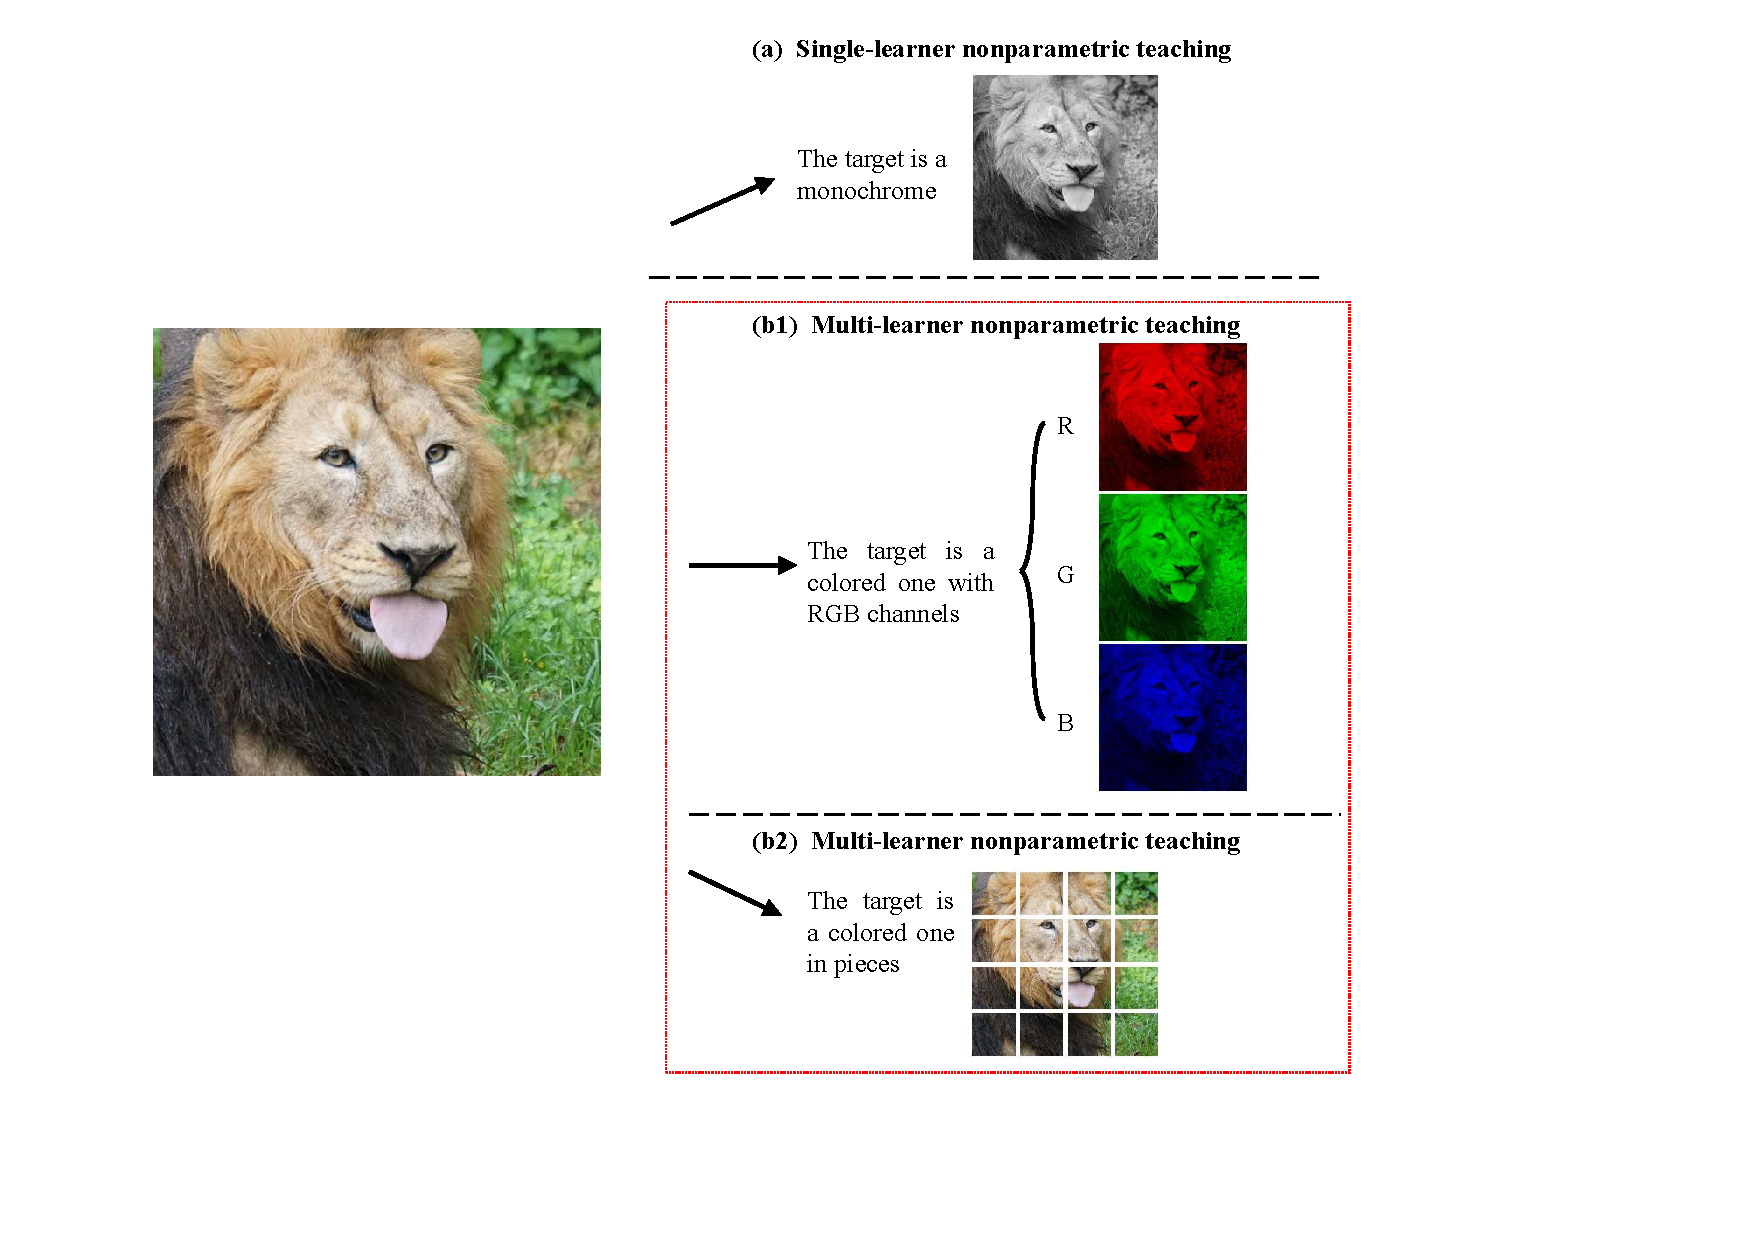
\includegraphics[width=0.8\textwidth]{comp.pdf}
      \caption{\footnotesize Comparison between the single-learner teaching and MINT.}
    \end{figure}    
\end{column}

\end{columns}
\end{frame}


\begin{frame}{Cont.}

{\bf \color{blue} Main Contribution}: 
\begin{itemize}
\justifying
\item By analyzing general \alert{vector-valued RKHS}, we study the {\bf multi-learner nonparametric teaching} (MINT), where the teacher selects examples based on a \alert{vector-valued target function} (each component of it is a scalar-valued one for a single learner) such that \alert{multiple} learners can learn its components simultaneously in a fast speed. 
\item Allowing the \alert{communication} across multiple learners, that is, learners are allowed to carry out \alert{linear combination} on current learnt functions of all learners, we investigate a communicated MINT where the teacher not only selects examples but also constructs a \alert{matrix} as the guide of communication in each iteration. 
\item Under a mild assumption, we \alert{theoretically} prove the efficiency of our \alert{multi-learner generalization} of nonparametric teaching. We also \alert{empirically} demonstrate its applicability and efficiency in extensive multi-learner experiments.
\end{itemize}
\end{frame}
%------------------------------------------------
\subsection{Teaching Settings}
\begin{frame}{Teaching Settings}

{\bf \color{blue} Vector-valued Functional Optimization}: We define multi-learner noparametric teaching as a \alert{vector-valued functional minimization} over the collection of potential teaching sequences $\mathbb{D}$ in the vector-valued reproducing kernel Hilbert space:
\begin{equation}\label{eq1}
\bm{\mathcal{D}}^*=\underset{\bm{\mathcal{D}}\in\mathbb{D}^d}{\arg\min}\quad \mathcal{M}(\hat{\bm{f}^*},\bm{f}^*)+\lambda\cdot \text{len}(\bm{\mathcal{D}}) \qquad \text{s.t.}\quad\hat{\bm{f}^*}=\mathcal{A}(\bm{\mathcal{D}})
\end{equation}
where $\mathcal{M}$ denotes a discrepancy measure, $\text{len}(\bm{\mathcal{D}})$, 
which is regularized by a constant $\lambda$, is the length of the teaching sequence $\bm{\mathcal{D}}$, and $\mathcal{A}$ represents the learning algorithm of learners. Specifically, $\mathcal{A}$ is taken as $\hat{\bm{f}^*}=\underset {\bm{f}\in\mathcal{H}^d}{\arg\min}\,\mathbb{E}_{(\bm{x},\bm{y})}\left[\mathcal{L}(\bm{f}(\bm{x}),\bm{y})\right]$,
where $(\bm{x},\bm{y})\in\mathcal{X}^d\times\mathcal{Y}^d$ and $(\bm{x},\bm{y})\sim[\mathbb{Q}_i(x_i,y_i)]^d$. Evaluated at an example vector $(\bm{x},\bm{y})=[(x_{i,j_i},y_{i,j_i})]^d$ with the example index $j_i\in\mathbb{N}_k$, the \alert{multi-learner convex} loss $\mathcal{L}$ therein is
$\mathcal{L}(\bm{f}(\bm{x}),\bm{y})=\sum_{i=1}^d \mathcal{L}_i(f_i(x_{i,j_i}),y_{i,j_i})=E_{\bm{x}}\left[[\mathcal{L}_i(f_i,y_{i,j_i})]^d\right]$, where $\mathcal{L}_i$ is the \alert{convex} loss for $i$-th learner.
\end{frame}

\begin{frame}{Cont.}

We investigate MINT in the \alert{gray-box setting}, which is equivalent to the one considered in \cite{Zhang2023NIMT}. To facilitate the theoretical analysis, we adopt some moderate \alert{assumptions regarding $\mathcal{L}_i$ and kernels}, which align with those made in \cite{Zhang2023NIMT}.

\begin{block}{Assumption 1}
	\label{lls}
	Each loss $\mathcal{L}_i(f_i), i\in\mathbb{N}_d$ is $L_{\mathcal{L}_i}$-Lipschitz smooth, \ie, $\forall f_i,f_i'\in\mathcal{H}$, $x_i\in\mathcal{X}$ and $i\in\mathbb{N}_d$ $$\left|E_{x_i}\left[\nabla_f \mathcal{L}_i(f_i)\right]-E_{x_i}\left[\nabla_f\mathcal{L}_i(f_i')\right]\right|\leq L_{\mathcal{L}_i} \left|E_{x_i}\left[f_i\right]-E_{x_i}\left[f_i'\right]\right|, $$ where $L_{\mathcal{L}_i}\geq0$ is a constant. To simplify the notation, we assume that $L_{\mathcal{L}_i}=L_\mathcal{L}$ for all $i\in\mathbb{N}_d$.
\end{block}

\begin{block}{Assumption 2}
	\label{bkf}
	Each kernel $K(x,x')\in\mathcal{H}$ is bounded, \ie, $\forall x,x' \in\mathcal{X},\,K(x,x')\leq M_K$, where $M_K\geq0$ is a constant.
\end{block}

\end{frame}

\subsection{Vanilla Multi-learner Teaching}

\begin{frame}{Vanilla Multi-learner Teaching}

In tackling MINT, we begin by examining a basic scenario in which \alert{multiple} learners \alert{concurrently} learns corresponding components of a vector-valued target function \alert{without communication} between them \cite{kakade2012regularization,cesamultitask}.

\begin{block}{Lemma 3 (Sufficient Descent for multi-learner RFT)}
Suppose there are $d$ learners, and the example \alert{mean} for each learner is $\mu_i=\mathbb{E}_{x_i\sim\mathbb{P}_i(x_i)}(x_i)<\infty$, and the \alert{variance} $\sigma_i^2=\mathbb{E}_{x_i\sim\mathbb{P}_i(x_i)}(x_i-\mu_i)^2<\infty, i\in\mathbb{N}_d$. Under the \alert{Lipschitz smooth and bounded kernel assumptions}, if $\eta^t_i\leq \frac{1}{2L_\mathcal{L}\cdot M_K}$ for all $i\in\mathbb{N}_d$, then RFT teachers can, \alert{on average}, reduce the multi-learner loss $\mathcal{L}(\bm{f})$ by:
\begin{eqnarray}
\resizebox{.94\hsize}{!}{		$\mathbb{E}_{\bm{x}\sim[\mathbb{P}_i(x_i)]^d}\left[\mathcal{L}(\bm{f}^{t+1})-\mathcal{L}(\bm{f}^t)\right]\leq-\frac{\tilde{\eta}^t}{2}\sum_{i=1}^d (m_{i,t}(\mu_i)+\frac{m_{i,t}''(\mu_i)}{2}\sigma_i^2)\leq-\frac{\tilde{\eta}^t d}{2}\cdot\min_{i\in\mathbb{N}_d} \left(m_{i,t}(\mu_i)+\frac{m_{i,t}''(\mu_i)}{2}\sigma_i^2\right)$},
\end{eqnarray}
where $\tilde{\eta}^t=\min_{i\in\mathbb{N}_d}\eta^t_i$ and $m_{i,t}(\dot{x})\mathrel{\mathop:}= E_{\dot{x}}[(\left.\nabla_f\mathcal{L}_i(f)\right|_{f=f^{t}_i})^2]$.
\end{block}

\end{frame}

\begin{frame}{Cont.}
\begin{block}{Theorem 4 (Convergence for multi-learner RFT)}    
Suppose the \alert{vector-valued} model for multiple learners is initialized with $\bm{f}^0\in\mathcal{H}^d$ and returns $\bm{f}^t\in\mathcal{H}^d$ after $t$ iterations, we have the \alert{upper bound} of $\min_{i\in\mathbb{N}_d} \left(m_{i,t}(\mu_i)+m_{i,t}''(\mu_i)\sigma_i^2/2\right)$ w.r.t. $t$:
	\begin{eqnarray}\label{eqcpft}
		\min_{i\in\mathbb{N}_d} \left(m_{i,t-1}(\mu_i)+m_{i,t-1}''(\mu_i)\sigma_i^2/2\right)\leq2\mathbb{E}_{\bm{x}\sim[\mathbb{P}_i(x_i)]^d}\left[\mathcal{L}(\bm{f}^0)\right]/(d\dot{\eta}t),
	\end{eqnarray}
	where $0<\dot{\eta}=\underset{l\in\{0\}\bigcup\mathbb{N}_{t-1}}{\min}\,\tilde{\eta}^l\leq 1/(2L_\mathcal{L}\cdot M_K)$, and given a small constant $\epsilon>0$ it would take approximately $\mathcal{O}\left(2(\mathbb{E}_{\bm{x}\sim[\mathbb{P}_i(x_i)]^d}\left[\mathcal{L}(\bm{f}^0)\right]-\epsilon)/(d\dot{\eta}\min_{i\in\mathbb{N}_d} \left(m_{i,t-1}(\mu_i)+m_{i,t-1}''(\mu_i)\sigma_i^2/2\right))\right)$ iterations to reduce the \alert{multi-learner} loss $\mathcal{L}$ to a \alert{sufficiently small} value and to reach a \alert{stationary point} in terms of $\mathcal{L}$.
\end{block} 
\end{frame}

\begin{frame}{Cont.}
\begin{block}{Lemma 5 (Sufficient Descent for multi-learner GFT)} Under the same assumption, if $\eta^t_i\leq \frac{1}{2L_\mathcal{L}\cdot M_K}$ for all $i\in\mathbb{N}_d$, the GFT teachers can achieve a \alert{greater} reduction in the multi-learner loss $\mathcal{L}$:
	\begin{eqnarray}
		\mathbb{E}_{\bm{x}\sim[\mathbb{P}_i(x_i)]^d}\left[\mathcal{L}(\bm{f}^{t+1})-\mathcal{L}(\bm{f}^t)\right]\leq-\frac{\tilde{\eta}^t}{2}\sum_{i=1}^d m_{i,t}({x^t_i}^*)\leq-\frac{\tilde{\eta}^t d}{2}\cdot\min_{i\in\mathbb{N}_d} m_{i,t}({x^t_i}^*),
	\end{eqnarray}
	where $\tilde{\eta}^t$ and $m_{i,t}(\cdot)$ retain their previous meaning.
\end{block} 
\end{frame}

\begin{frame}{Cont.}
\begin{block}{Theorem 6 (Convergence for multi-learner GFT)} Suppose the \alert{vector-valued} model for multiple learners is initialized with $\bm{f}^0\in\mathcal{H}^d$ and returns $\bm{f}^t\in\mathcal{H}^d$ after $t$ iterations, we have the \alert{upper bound} of $\min_{i\in\mathbb{N}_d} m_{i,t}({x^t_i}^*)$ w.r.t. $t$:
	\begin{eqnarray}\label{eqcgft}
		\min_{i\in\mathbb{N}_d} m_{i,t-1}({x^{t-1}_i}^*)\leq\frac{2}{d\dot{\eta}t}\mathbb{E}_{\bm{x}\sim[\mathbb{P}_i(x_i)]^d}\left[\mathcal{L}(\bm{f}^0)\right]+\frac{1}{d}\sum_{l=0}^{t-1}\sum_{i=1}^d \left(\|{x^l_i}^*-\mu_i\|_2\right),
	\end{eqnarray}
	where $\dot{\eta}$ has the same definition as before, and given a small constant $\epsilon>0$ it would need around $\mathcal{O}\left(2(\mathbb{E}_{\bm{x}\sim[\mathbb{P}_i(x_i)]^d}\left[\mathcal{L}(\bm{f}^0)\right]-\epsilon)/(d\dot{\eta}\min_{i\in\mathbb{N}_d} m_{i,t-1}({x^{t-1}_i}^*))\right)$ iterations to decrease the \alert{multi-learner} loss $\mathcal{L}$ to a \alert{sufficiently small} value and to reach a \alert{stationary point} in terms of $\mathcal{L}$.
\end{block} 
\end{frame}
%------------------------------------------------
\subsection{Communicated Multi-learner Teaching}
\begin{frame}{Communicated Multi-learner Teaching}
An infant would \alert{integrate} previously learnt knowledge to grasp a new target concept, such as comprehending  what a zebra is by combining the learnt ideas of horses and black-and-white stripes. Such an efficient paradigm motivates us to explore the \alert{communicated MINT}, which enables the \alert{communication} between learners.
\begin{block}{Proposition 5}
    If the proximity between $\bm{f}^t$ and $\bm{f}^*$ is \alert{sufficiently close}, meaning that $\|\bm{f}^t-\bm{f}^*\|_{\mathcal{H}^d}\leq\epsilon$ where $\epsilon$ is a tiny positive constant, then $A^t$ equals the \alert{identity matrix} $I_d$.
\end{block}

\begin{block}{Lemma 6}
    Under \alert{Lipschitz smooth} assumption, the \alert{communication} across learners will result in a \alert{reduction} of the \alert{multi-learner convex} loss $\mathcal{L}$ by  $0\leq\mathcal{L}(\bm{f}^t)-\mathcal{L}(A^t\bm{f}^t)\leq2L_\mathcal{L}\|\bm{f}^t-\bm{f}^*\|_{\mathcal{H}^d}$.
\end{block}
\end{frame}



\begin{frame}{Cont.}
\begin{block}{Theorem 7}
    Suppose the \alert{communication} in the $t$-th iteration of multiple learners is denoted by the \alert{matrix} $A^t$ and returns $\bm{f}^{t+1}_{A^t}\in\mathcal{H}^d$, for both RFT and GFT we have:
	$$\mathbb{E}_{\bm{x}\sim[\mathbb{P}_i(x_i)]^d}\left[\mathcal{L}(\bm{f}^{t+1}_{A^t})-\mathcal{L}(\bm{f}^t)\right]\leq
		\mathbb{E}_{\bm{x}\sim[\mathbb{P}_i(x_i)]^d}\left[\mathcal{L}(\bm{f}^{t+1}_{A^t})-\mathcal{L}(A^t\bm{f}^t)\right]\leq0.$$
\end{block} 
\end{frame}

%------------------------------------------------
\section{Experiments and Results}
\begin{frame}{Experiments and Results}

\justify
Testing the teaching of a \alert{multi-learner (vector-valued) target model}, MINT presents more satisfactory performance than repeatedly carrying out the single-learner teaching, which is \alert{consistent with our theoretical findings}.

\vspace{1mm}
\begin{itemize}
    \item {\bf MINT in gray scale.}
\end{itemize}
\centering
\begin{tabular}{lclc}
{\scriptsize \color{blue} Simultaneous teaching of a tiger and a cheetah.} \vspace{-2mm}\\

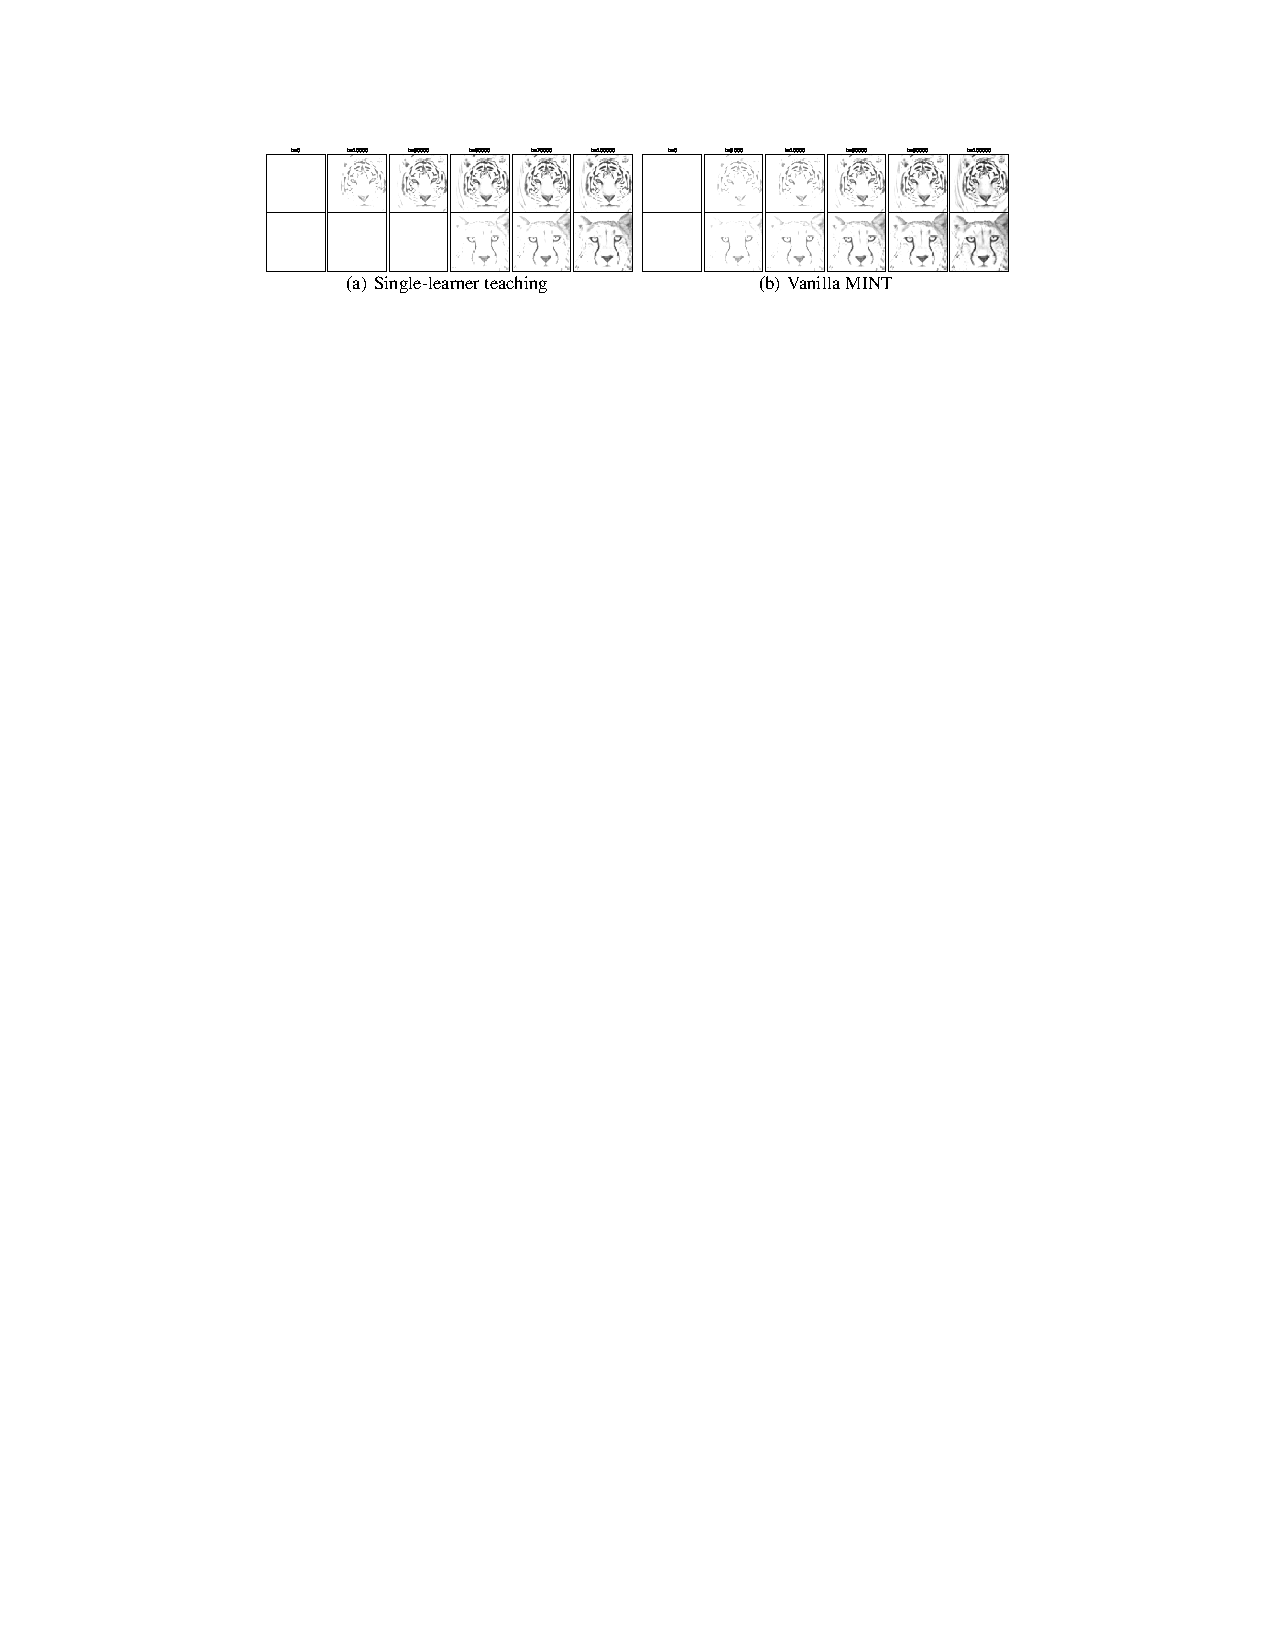
\includegraphics[width=0.85\linewidth]{./out/grayTigerCheetah}\\
{\scriptsize \color{blue} Teaching of a lion by partition.}\vspace{-1mm}\\

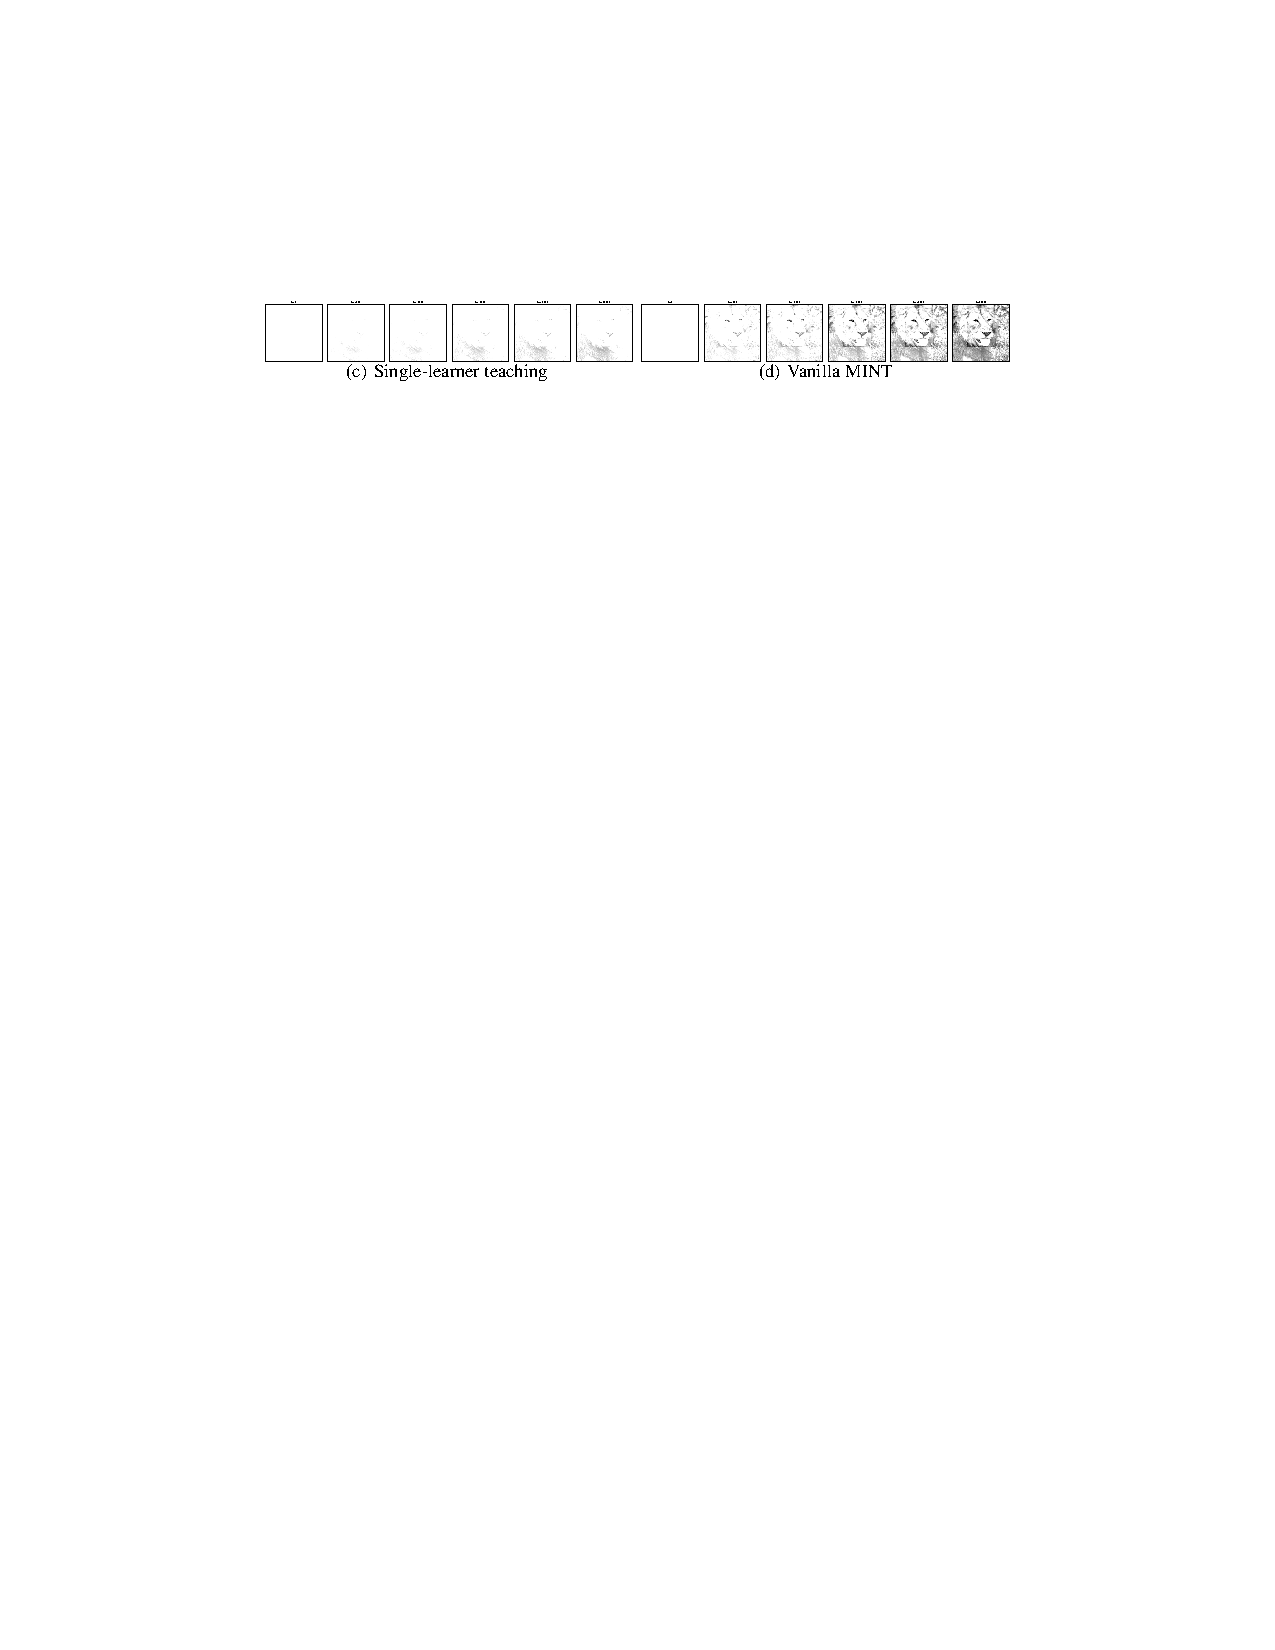
\includegraphics[width=0.85\linewidth]{./out/grayLion}\\
\end{tabular}

\end{frame}


\begin{frame}{Cont.}
\begin{itemize}
    \item {\bf  MINT in three (RGB) channels.}
\end{itemize}

\centering
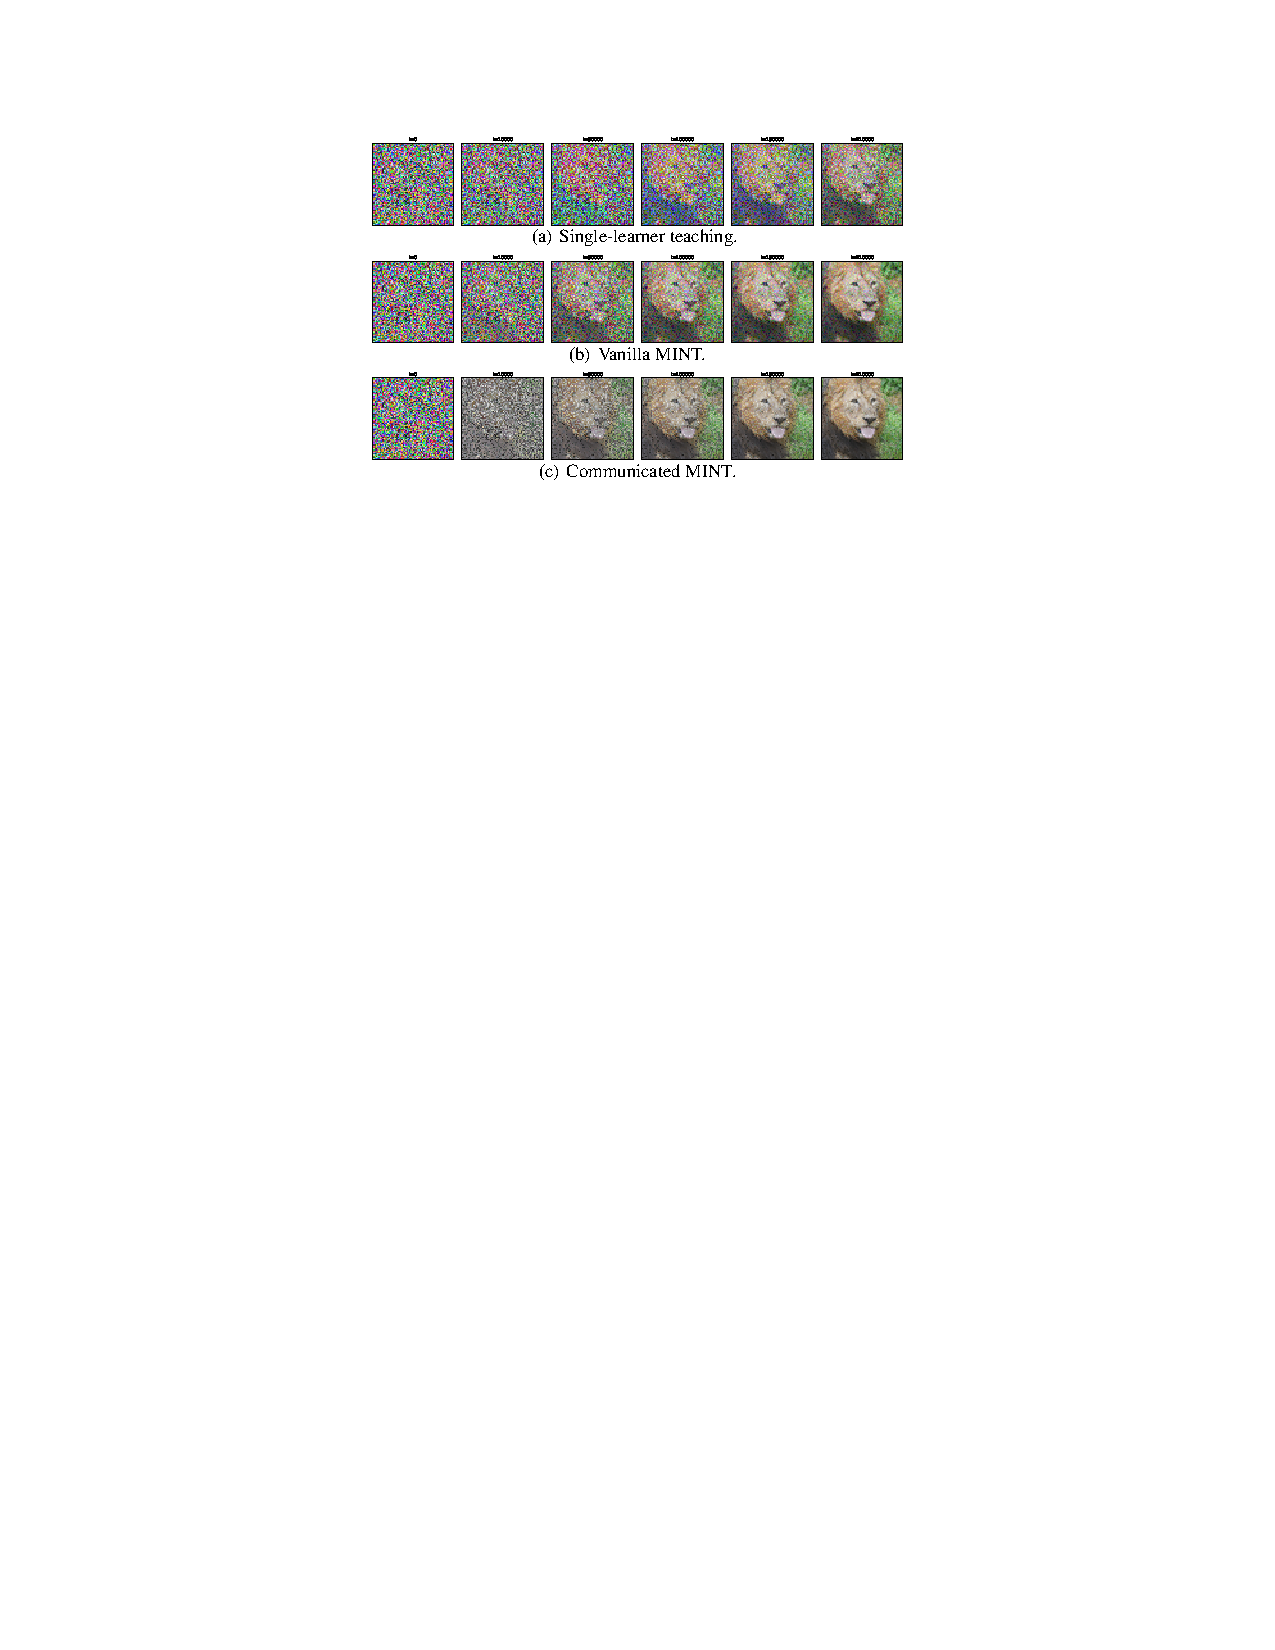
\includegraphics[width=0.7\linewidth]{./out/RGBlion}

\end{frame}

%------------------------------------------------

\begin{frame}
    \Huge{\centerline{\textbf{Thank you for listening!}}}
\end{frame}

%------------------------------------------------
\begin{frame}[allowframebreaks]
    \frametitle{References}
    \bibliographystyle{plain}
    {\footnotesize \bibliography{ref.bib}}
\end{frame}

%----------------------------------------------------------------------------------------
\end{document}